\section{Trapezoidal}
\begin{figure}[h]
\centering
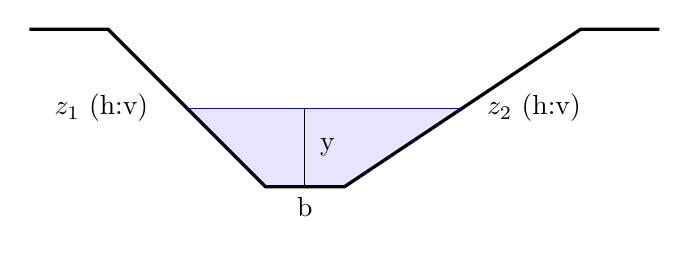
\begin{tikzpicture}
\draw[very thick] (0,0) -- (1,0) -- node[left=10pt]{$z_1$ (h:v)}(3,-2)--node[below]{b}(4,-2)--node[right=5]{$z_2$ (h:v)} (7,0) -- (8,0);
\draw[blue] (2,-1) -- (5.5,-1);
\filldraw[fill=blue, opacity=0.1](2, -1) --(5.5, -1) -- (4, -2) -- (3, -2);

\draw (3.5,-2)--node[right=2]{y} (3.5,-1);
\end{tikzpicture}
\caption{Trapezoidal Section}
\end{figure}

\begin{equation}
A = \frac{1}{2} (z_1 + z_2) y^2 + by
\end{equation}

\begin{equation}
P = \left(\sqrt{1+z_1^2} + \sqrt{1+z_2^2}\right)y + b
\end{equation}

\begin{equation}
\frac{\partial A}{\partial y} = (z_1 + z_2)y + b
\end{equation}

\begin{equation}
\frac{\partial ^2A}{\partial y^2} = z_1 + z_2
\end{equation}

\begin{equation}
\frac{dP}{dy} = \sqrt{1+z_1^2} + \sqrt{1+z_2^2}
\end{equation}

